\documentclass{article}

% if you need to pass options to natbib, use, e.g.:
%     \PassOptionsToPackage{numbers, compress}{natbib}
% before loading neurips_2023

% ready for submission
\usepackage[final]{neurips_2023}

% to compile a preprint version, e.g., for submission to arXiv, add add the
% [preprint] option:
%     \usepackage[preprint]{neurips_2023}

% to compile a camera-ready version, add the [final] option, e.g.:
%     \usepackage[final]{neurips_2023}

% to avoid loading the natbib package, add option nonatbib:
%    \usepackage[nonatbib]{neurips_2023}

\usepackage[utf8]{inputenc} % allow utf-8 input
\usepackage[T1]{fontenc}    % use 8-bit T1 fonts
\usepackage{hyperref}       % hyperlinks
\usepackage{url}            % simple URL typesetting
\usepackage{booktabs}       % professional-quality tables
\usepackage{amsfonts}       % blackboard math symbols
\usepackage{nicefrac}       % compact symbols for 1/2, etc.
\usepackage{microtype}      % microtypography
\usepackage{xcolor}         % colors
\usepackage{graphicx}
\title{Time Series Prediction Problem — Detect Future Values of Stock Prices of a Set of Companies}

% The \author macro works with any number of authors. There are two commands
% used to separate the names and addresses of multiple authors: \And and \AND.
%
% Using \And between authors leaves it to LaTeX to determine where to break the
% lines. Using \AND forces a line break at that point. So, if LaTeX puts 3 of 4
% authors names on the first line, and the last on the second line, try using
% \AND instead of \And before the third author name.

\author{%
Likhit Garimella$^1$ \quad Manasvini Nittala$^1$ \quad Sahithi Reddy Sakinala$^1$ \\
\textbf{Aniket Anvekar}$^1$ \quad \textbf{Jahnavi Manchala}$^1$ \\
$^1$Rutgers University \\
\texttt{\{lg836,mn777,ss4362,ava66,jm2658\}@rutgers.edu}\\
}

\begin{document}

\maketitle

\begin{abstract}
Recurrent Neural Networks (RNNs), specifically a variant with Long ShortTerm Memory (LSTM) and Gated Recurrent Unit (GRU), are enjoying renewed interest due to successful applications in a wide range of machine learning problems involving sequential data. However, while LSTMs and GRUs provide exceptional results in practice, the source of their performance and their limitations still need to be better understood. Using time series prediction models as an interpretable testbed, we aim to analyze the stock prices. In particular, our project focuses on the trends in stock prices. Moreover, our comparative analysis with vanilla RNN, LSTMs, and GRUs shows a better way of getting accurate stock price predictions. Finally, we analyze the remaining errors and suggest areas for further study.
\end{abstract}

\section{Introduction}

An artificial neural network that is adapted to handle time series data or data that consist of sequences is known as Recurrent Neural Networks (RNNs). Unlike feed-forward neural networks, which process inputs independently, RNNs maintain an internal state that allows them to process sequences of inputs and capture temporal dependencies.

\subsection{Simple RNN}
The simplest type of RNN also called as SimpleRNN, is based on the Elman network or the Jordan network.
A SimpleRNN has a basic architecture consisting of a single hidden layer that takes the input at each time step and produces an output and a hidden state fed back into the network at the next step. The hidden state serves as the memory of the network, allowing it to capture temporal dependencies in the sequence. However, Simple RNNs are known to suffer from the vanishing gradient problem, making it challenging to learn long-term dependencies.

\subsection{Long Short Term Memory (LSTMs)}
Long Short-Term Memory (LSTM) is a type of RNN designed to overcome the limitations of Simple RNNs. LSTM has a more complex architecture, consisting of memory cells and three gates: input, output, and forget gates. The memory cells store information over time, and the gates control the flow of information into and out of the cells. The input gate controls the extent to which new information is stored in the cells, while the output gate controls the extent to which the information produces an output. The forget gate controls the extent to which the previous memory is retained.

\subsection{Gated Recurrent Units (GRUs)}
Gated Recurrent Units (GRUs) are a simplified version of LSTM that use fewer parameters and are faster to compute. Like LSTM, GRUs also have memory cells and gates to control the flow of information. However, GRUs have only two gates: reset and update gates. The reset gate determines how to combine the new input with the previous memory, while the update gate determines how much of the previous memory to keep. GRUs have achieved comparable performance to LSTM on many tasks requiring less computation.

\section{Related Work}
\label{gen_inst}
\subsection{Problem Statement}
Time Series Prediction Problem: To predict the stock prices of S\&P 500 companies using RNN, LSTM and GRU models.

\section{Setup}
\label{headings}
Our project focuses on comparing simple RNN, LSTM, and GRU. Therefore, our setup is designed to be simple and the comparisons fair. They are evaluated on a stock prediction dataset of S\&P 500 companies from different domains to account for cross-domain variations.

\subsection{Datasets}
We used 2 datasets for training and testing.
\subsubsection {Training}
S\&P 500 dataset consisting of stock prices for 500 companies from January 1 2013 - December 31 2018. This dataset consists the prices on financial days only. It is a huge dataset with \~ 700,000 values
\subsubsection {Testing}
The test dataset consists of financial days of January 2019.

\subsection{Model}
We will implement simple RNN, LSTM, and GRU models. We will make models that capture the downward and upward trends of stock prices. 
\subsection{Approach}
Train the RNN, LSTM, and GRU models on stock price data from the beginning of 2013 to the end of 2018. Based on this training and the correlations identified, we will try to predict the first month of 2019.
\paragraph{Data Preprocessing} First check the dataset for any missing data and null values. Impute if any are found, and then normalise the data and extract the features.
\paragraph{Feature Scaling} 2 effective ways of applying feature scaling — standardisation and normalisation (equations). While building our RNN, we apply normalisation.Importing min max scaler class from Scikit learn library.Then apply normalisation, by getting the minimum stock price and maximum stock price from the input training set, to be able to apply it in the normalisation formula.Now, we get the normalised stock prices between 0 and 1 — the last value tends to go to 1 as the stock prices are increasing.
\paragraph{Timesteps}
At each time T, the RNN is going to look at the 60 stock prices before time T — that means, based on the stock prices between 60 days before time T and time T, the RNN will try to learn and understand the correlations and trends. And based on this, it will predict the next output, the stock price at time (T+1).
\section{Results}
\subsection{Conclusion}
We implemented RNN, LSTM, and GRU models to predict the stock prices of S\&P 500 companies from different domains to account for cross-domain variations. The graphs can be used to evaluate the accuracy of the machine learning models in predicting stock prices over time. If the predicted prices closely follow the actual prices, then it suggests that the model is accurate and can be used to make future predictions with some degree of confidence. On the other hand, if there are significant discrepancies between the predicted and actual prices, then it may suggest that the model needs to be improved or that external factors must be considered. Comparing all the above graphs, we observed that GRU outperforms LSTM and SimpleRNN in terms of accuracy, as the predicted stock prices are very much aligned with the actual prices.Below are the outputs we have obtained.
\subsection{Figures}
\begin{figure}[htp]
    \centering
    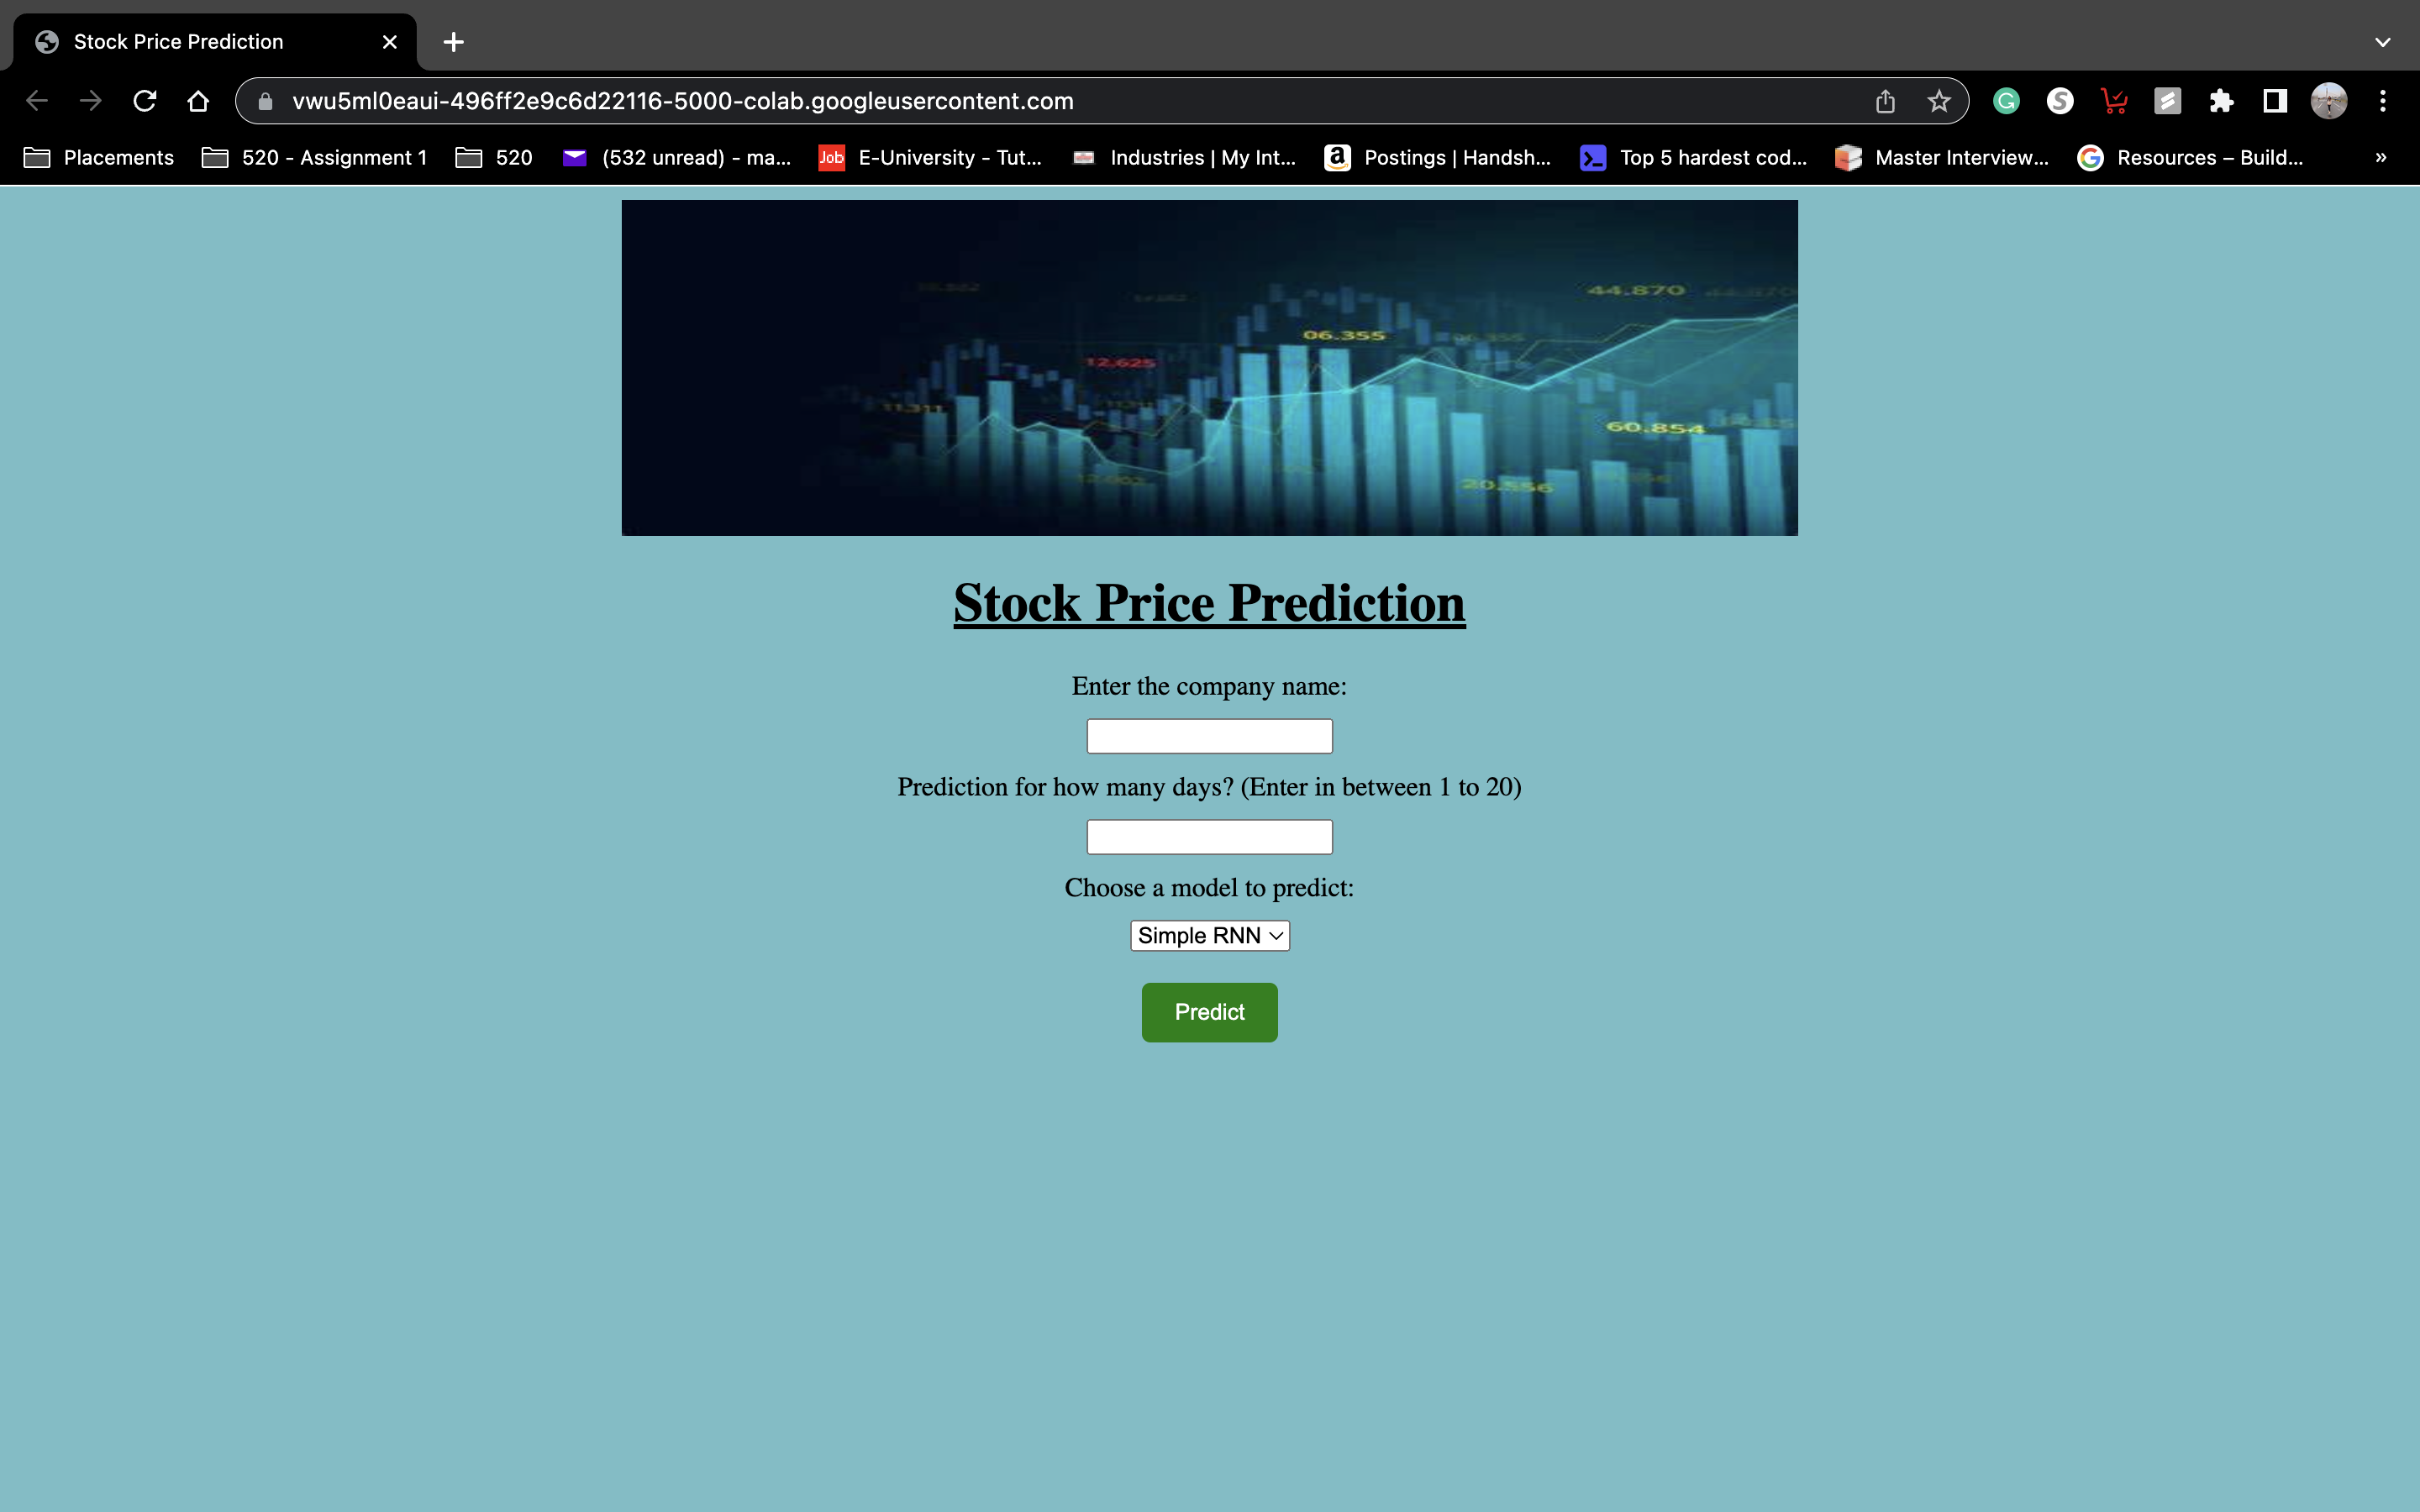
\includegraphics[width=10cm]{UI_MAIN.png}
    \caption{Main UI Page}
\end{figure}
\begin{figure}[htp]
    \centering
    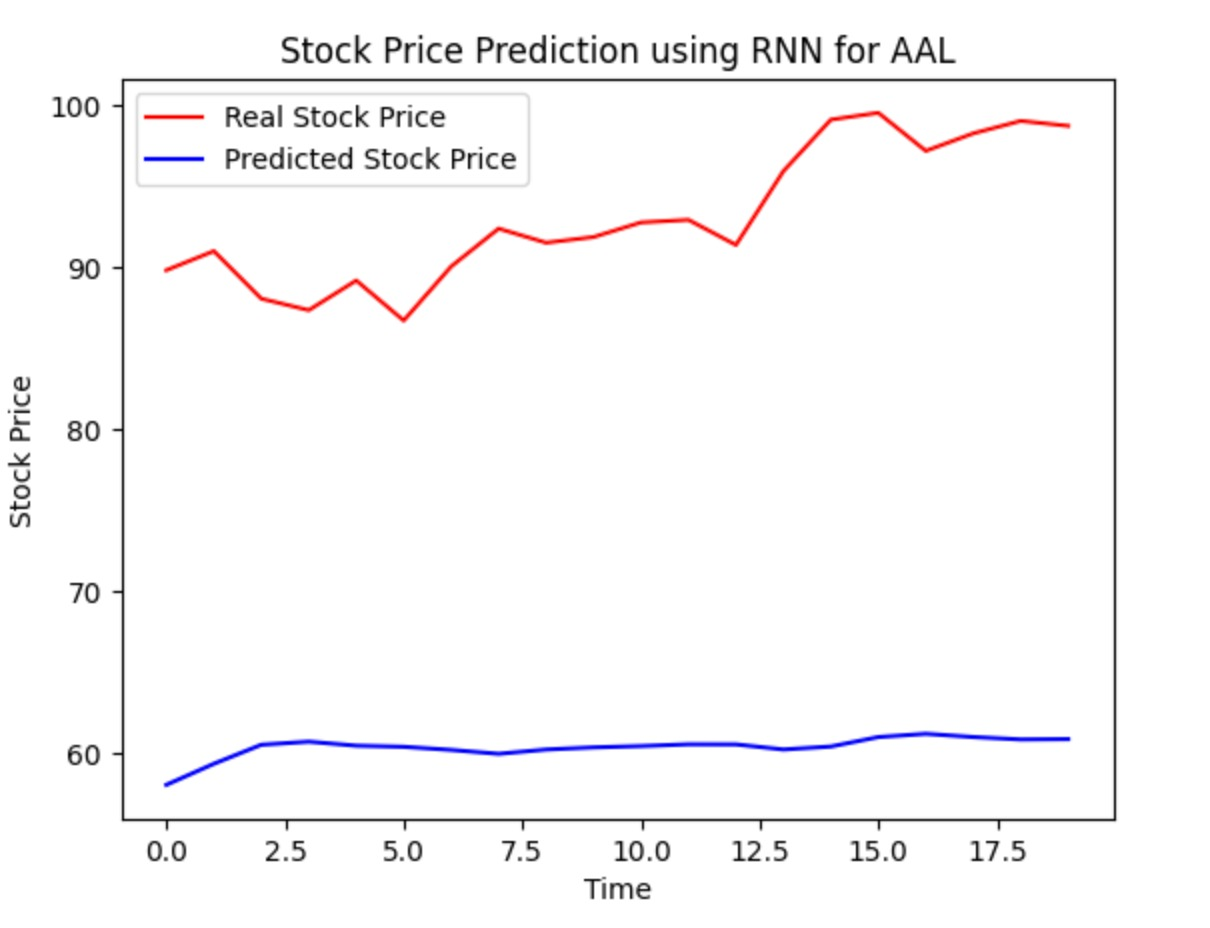
\includegraphics[width=6.5cm]{AAL_RNN.jpg}
    \caption{Stocks of American Airlines trained using RNN}
\end{figure}

\begin{figure}[htp]
    \centering
    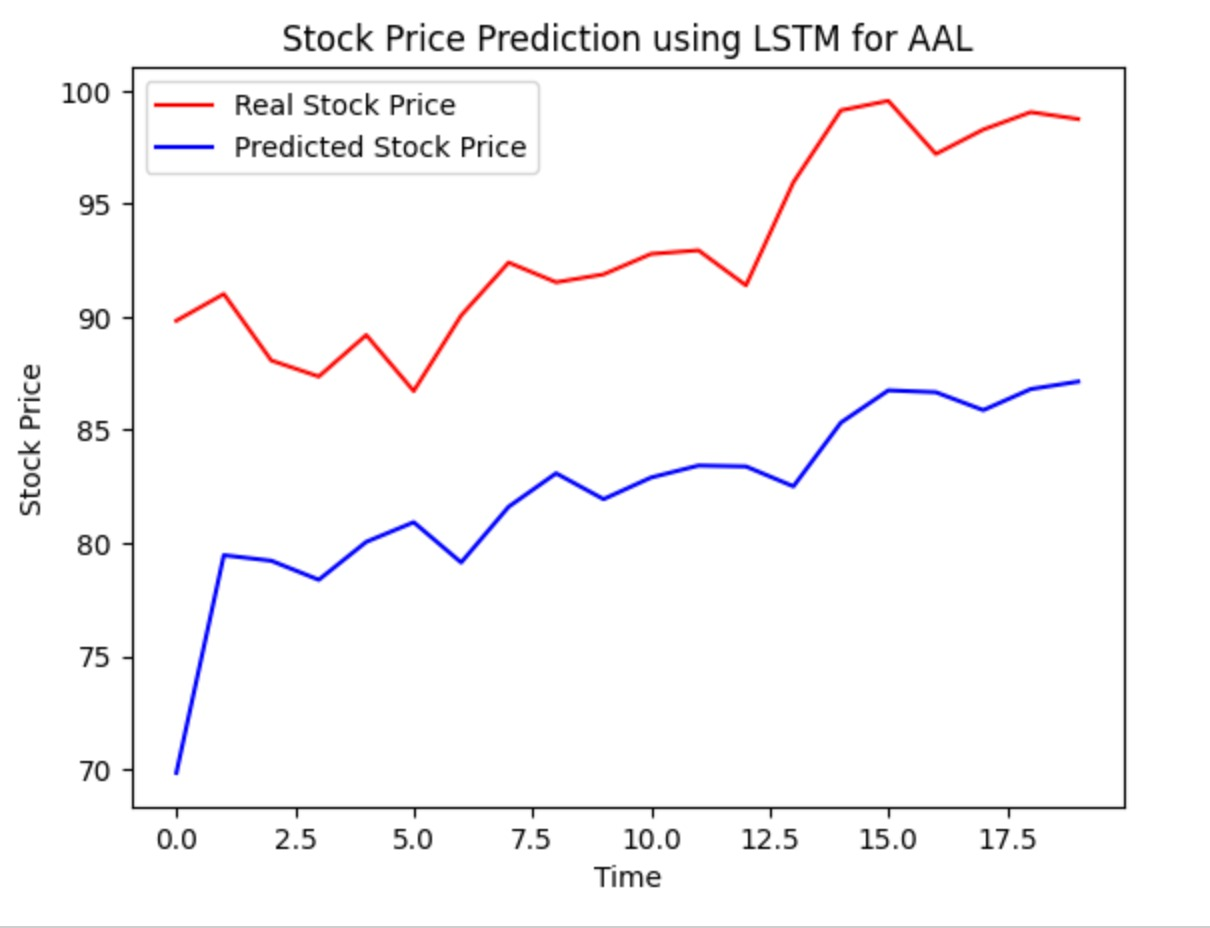
\includegraphics[width=6.5cm]{AAL_LSTM.jpg}
    \caption{Stocks of American Airlines trained using LSTM}
\end{figure}

\begin{figure}[htp]
    \centering
    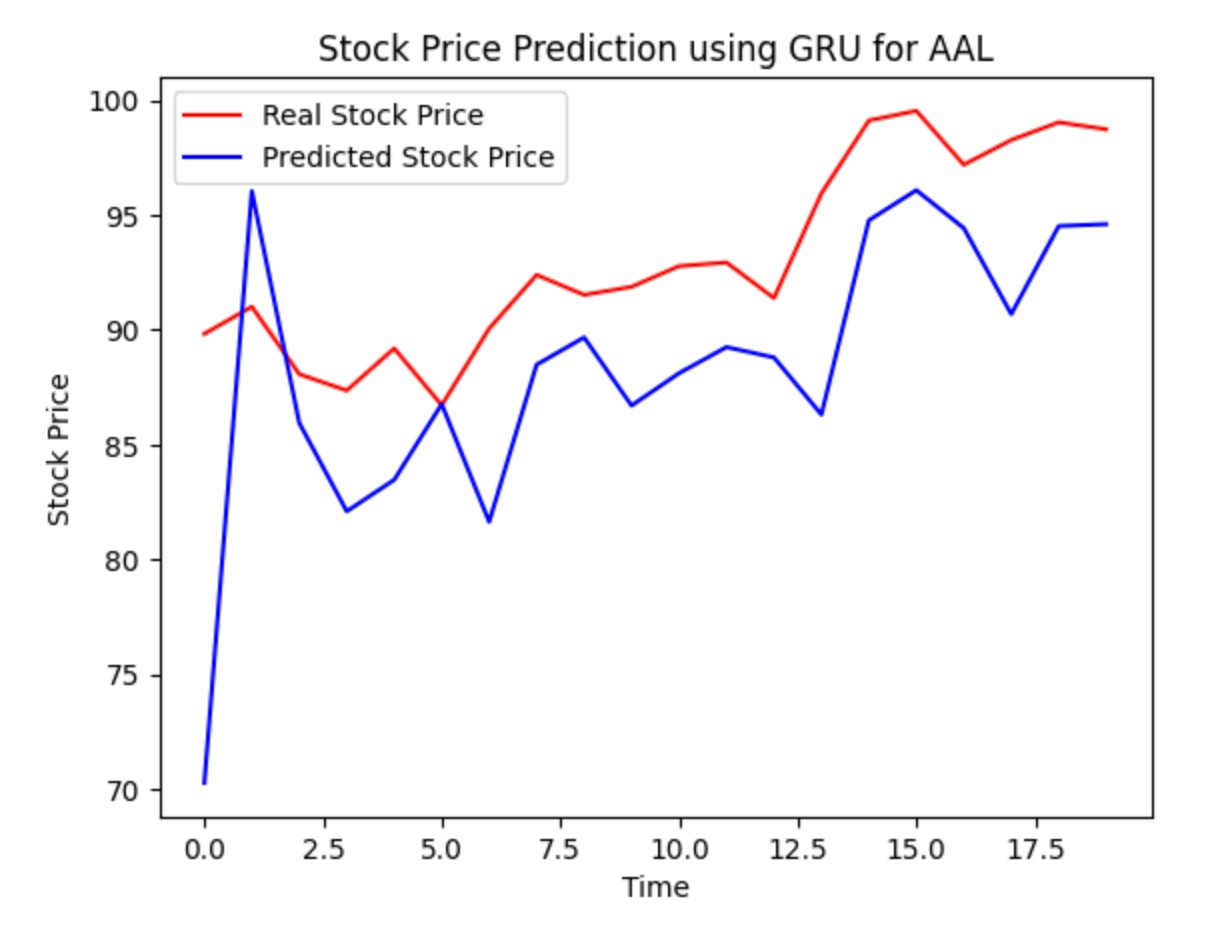
\includegraphics[width=6.5cm]{AAL_GRU.jpg}
    \caption{Stocks of American Airlines trained using GRU}
\end{figure}

\begin{figure}[htp]
    \centering
    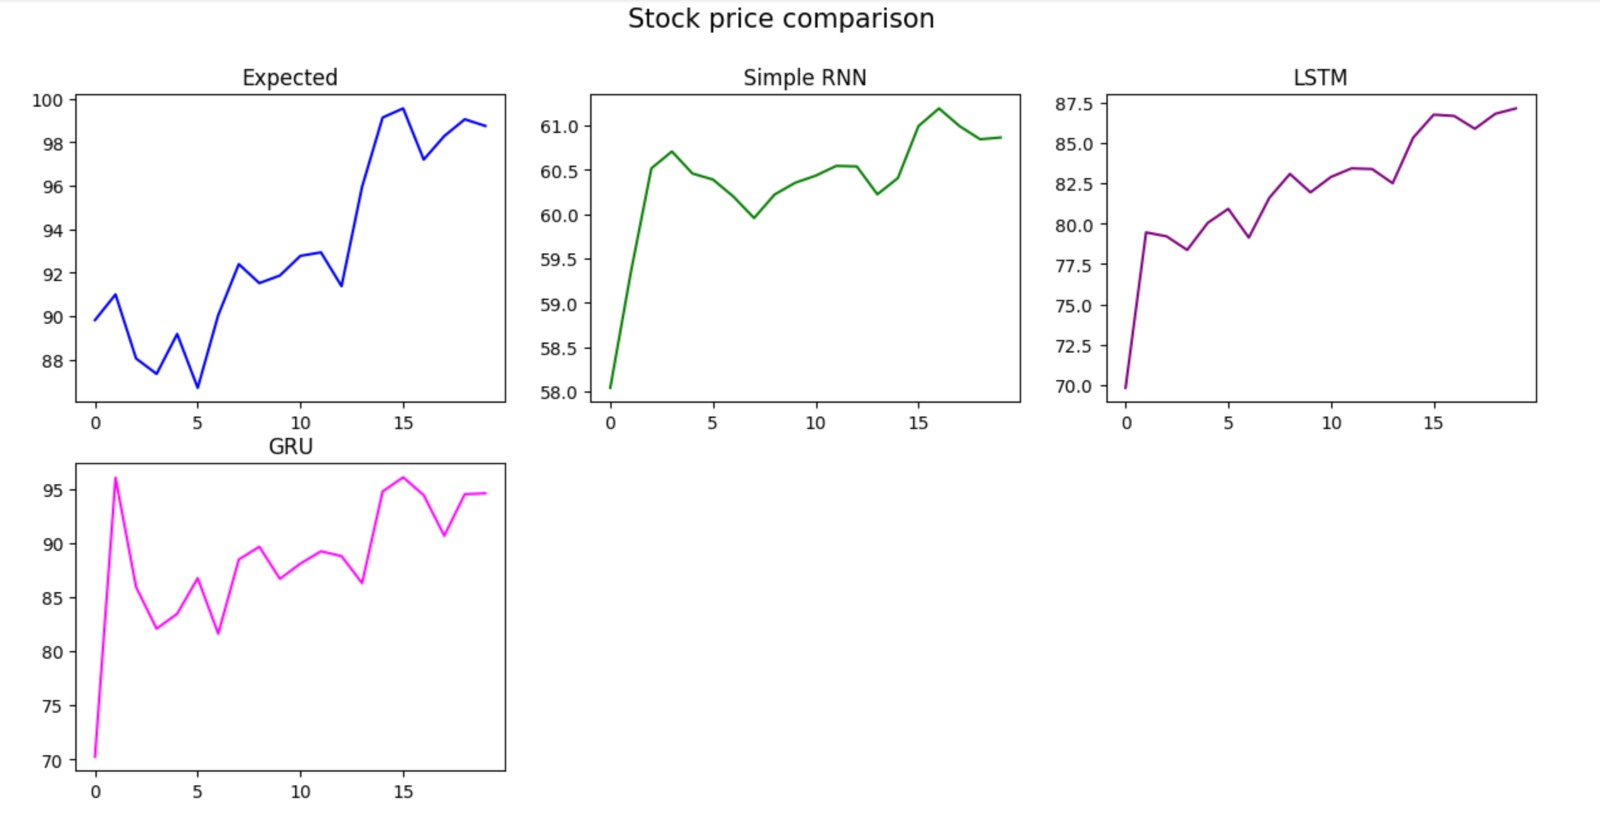
\includegraphics[width=8.5cm]{AAL_ALL.jpg}
    \caption{Comparing expected and obtained predictions}
\end{figure}

\begin{figure}[htp]
    \centering
    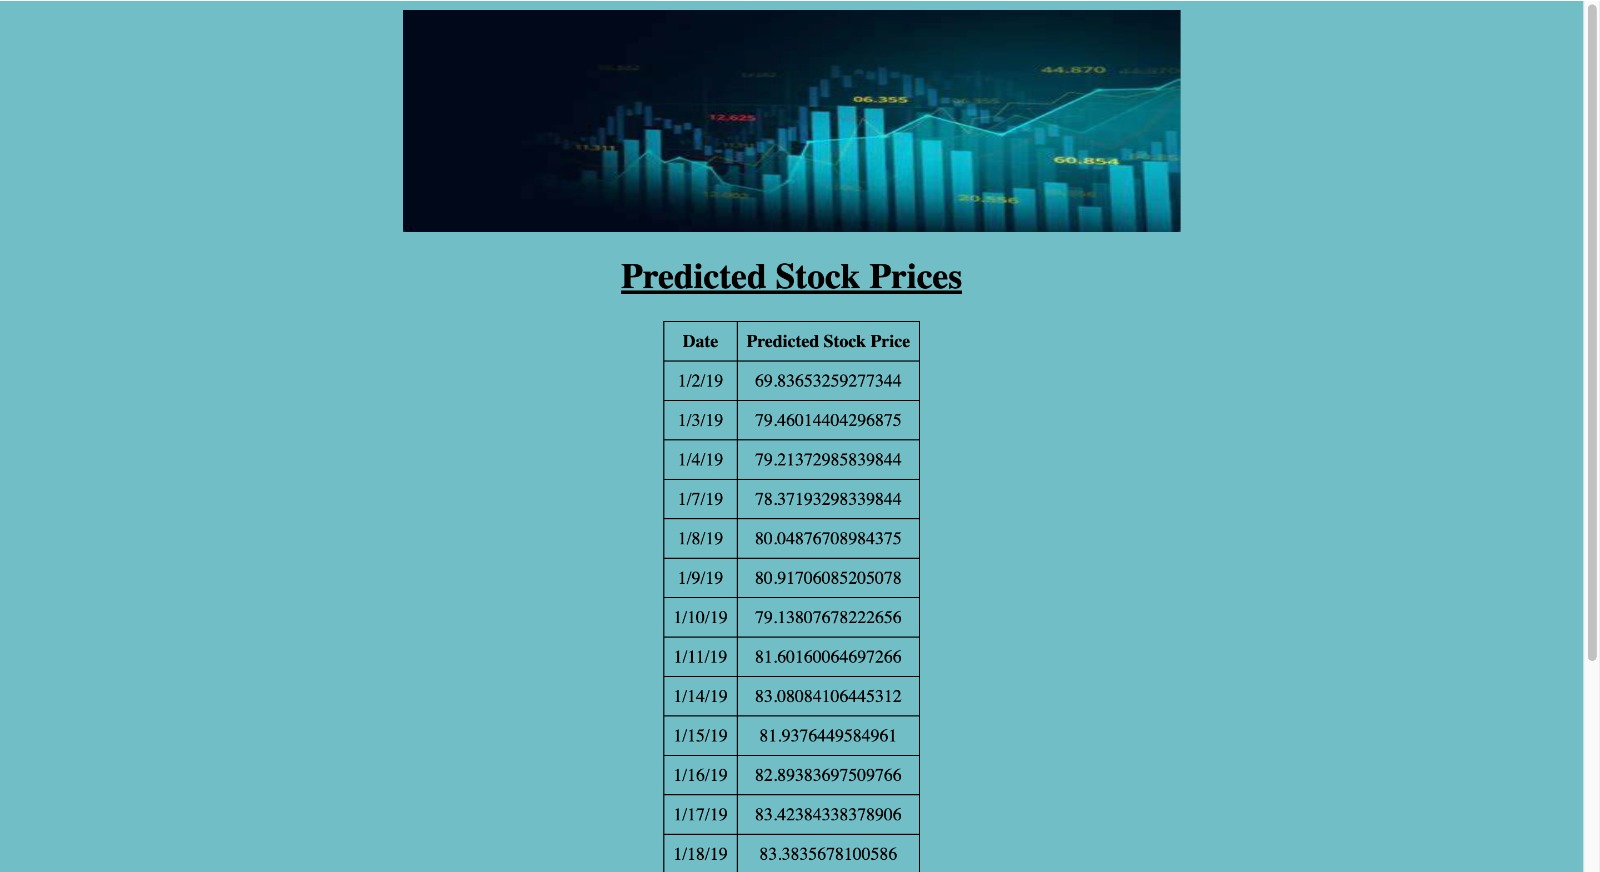
\includegraphics[width=10cm]{AAL_PRED.jpg}
    \caption{Predictions for American Airlines for selected model}
\end{figure}

\begin{figure}[htp]
    \centering
    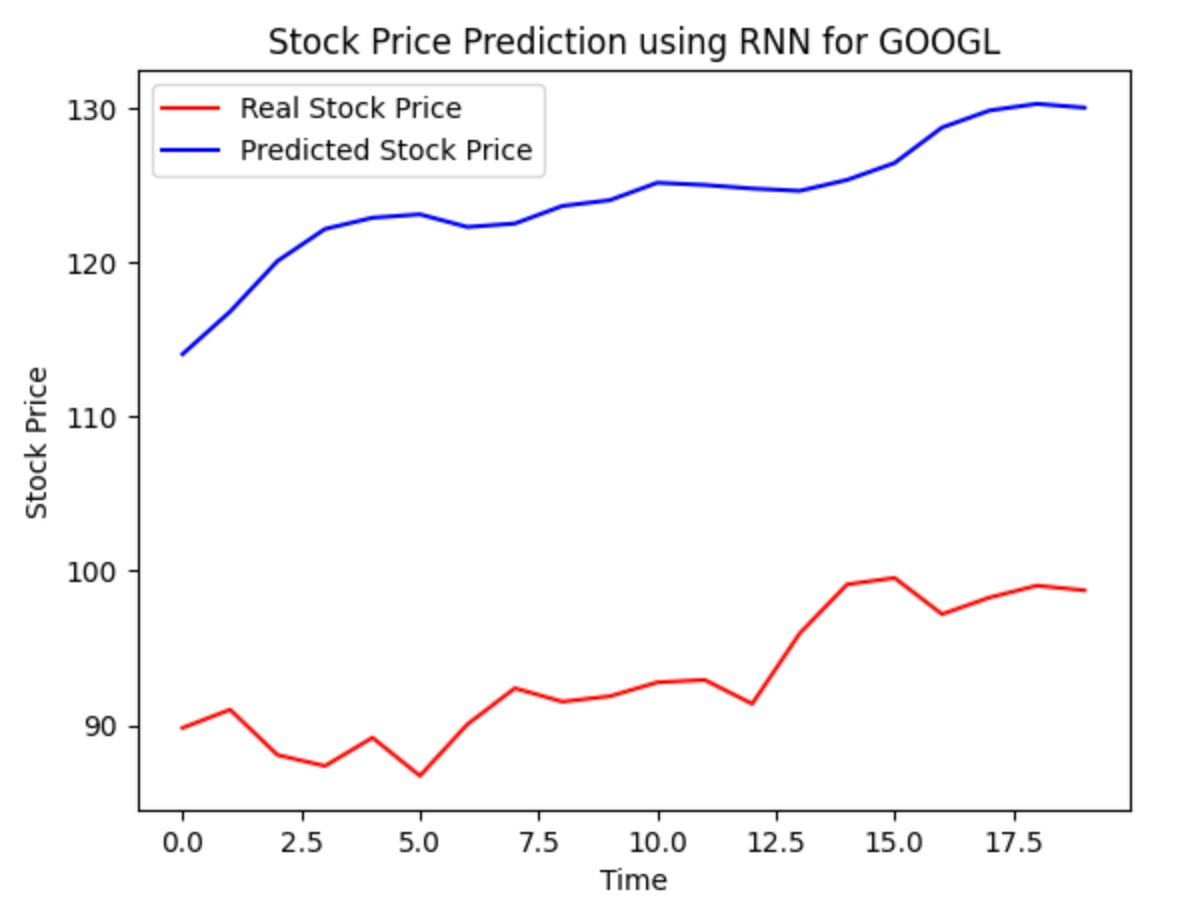
\includegraphics[width=6.5cm]{GOOGL_RNN.jpg}
    \caption{Stocks of Google trained using RNN}
\end{figure}

\begin{figure}[htp]
    \centering
    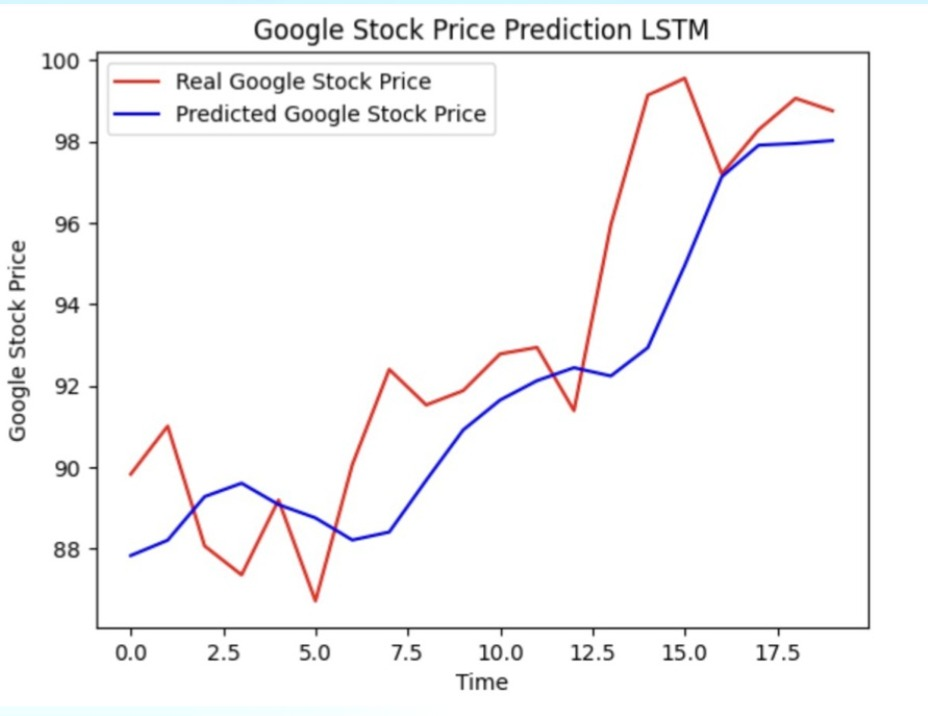
\includegraphics[width=6.5cm]{GOOGL_LSTM.jpg}
    \caption{Stocks of Google trained using LSTM}
\end{figure}

\begin{figure}[htp]
    \centering
    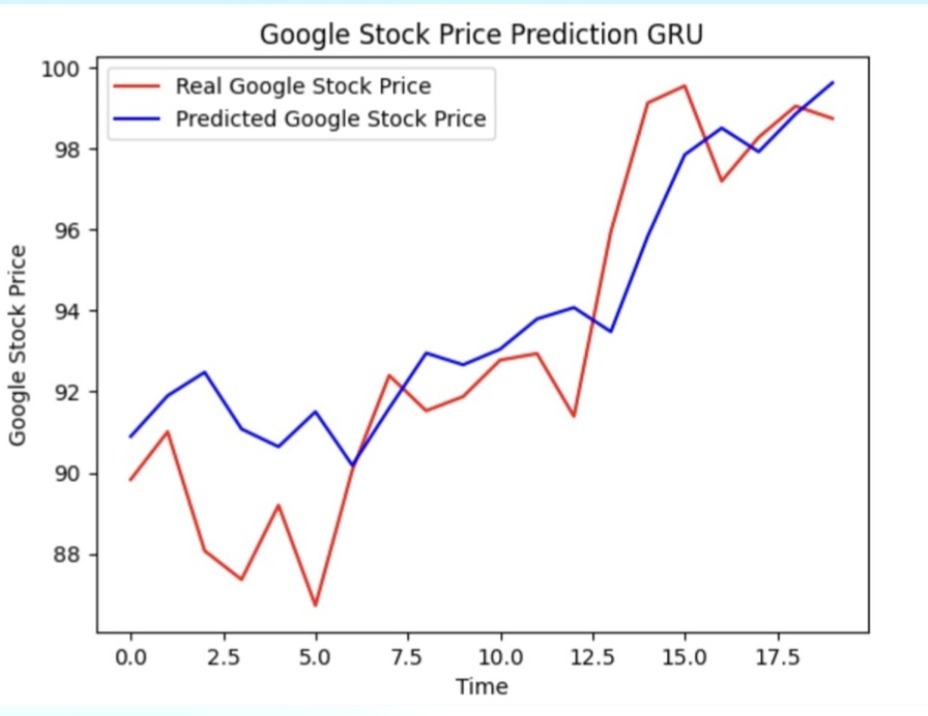
\includegraphics[width=6.5cm]{GOOGL_GRU.jpg}
    \caption{Stocks of Google trained using GRU}
\end{figure}
\begin{figure}[htp]
    \centering
    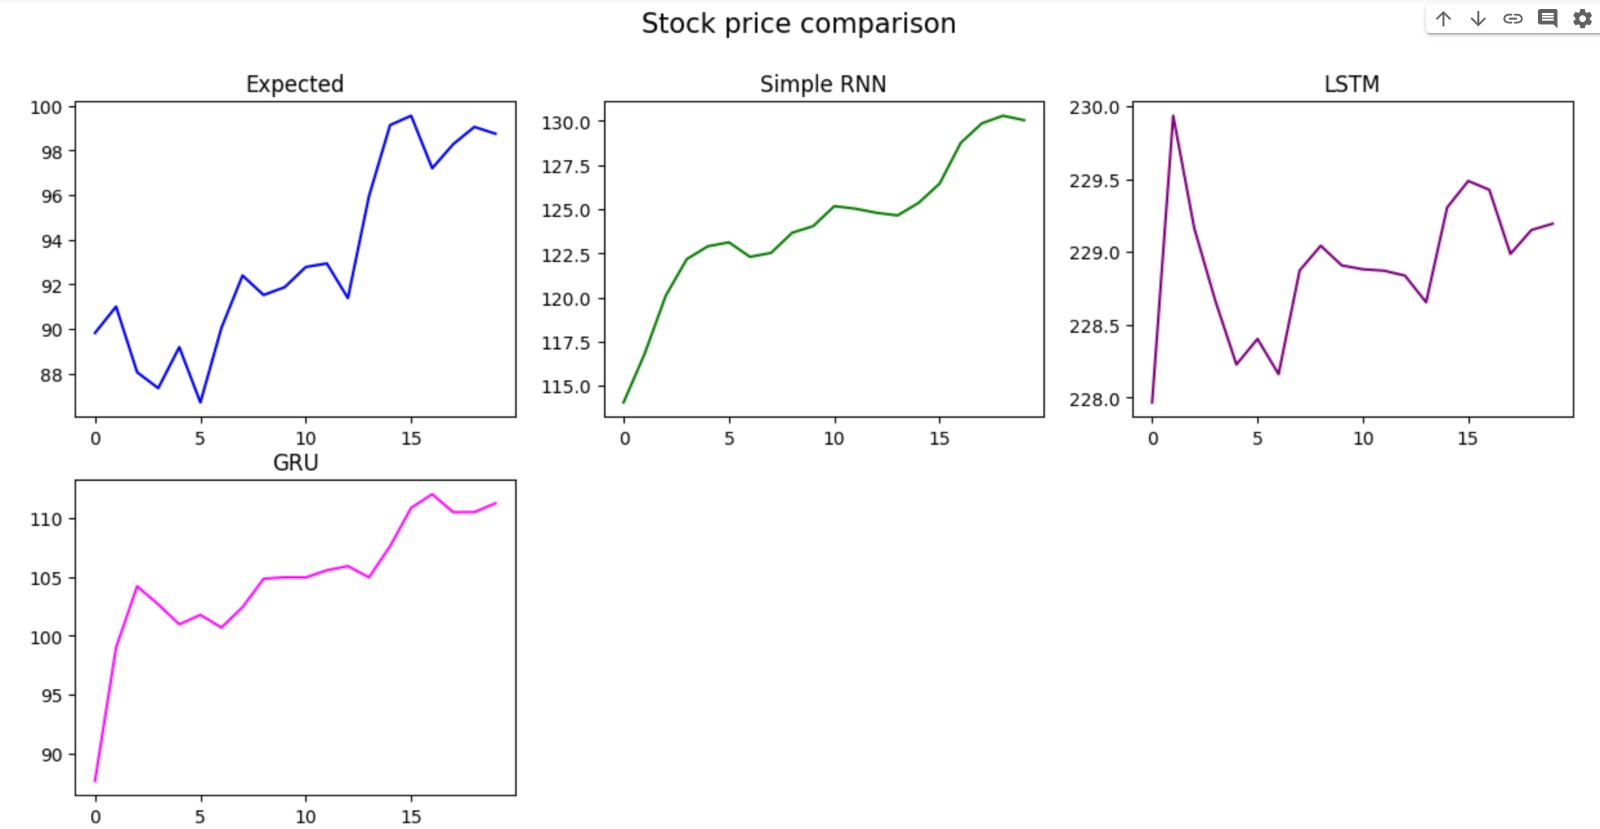
\includegraphics[width=8.5cm]{GOOGL_ALL.jpg}
    \caption{Comparing expected and obtained predictions}
\end{figure}
\begin{figure}[htp]
    \centering
    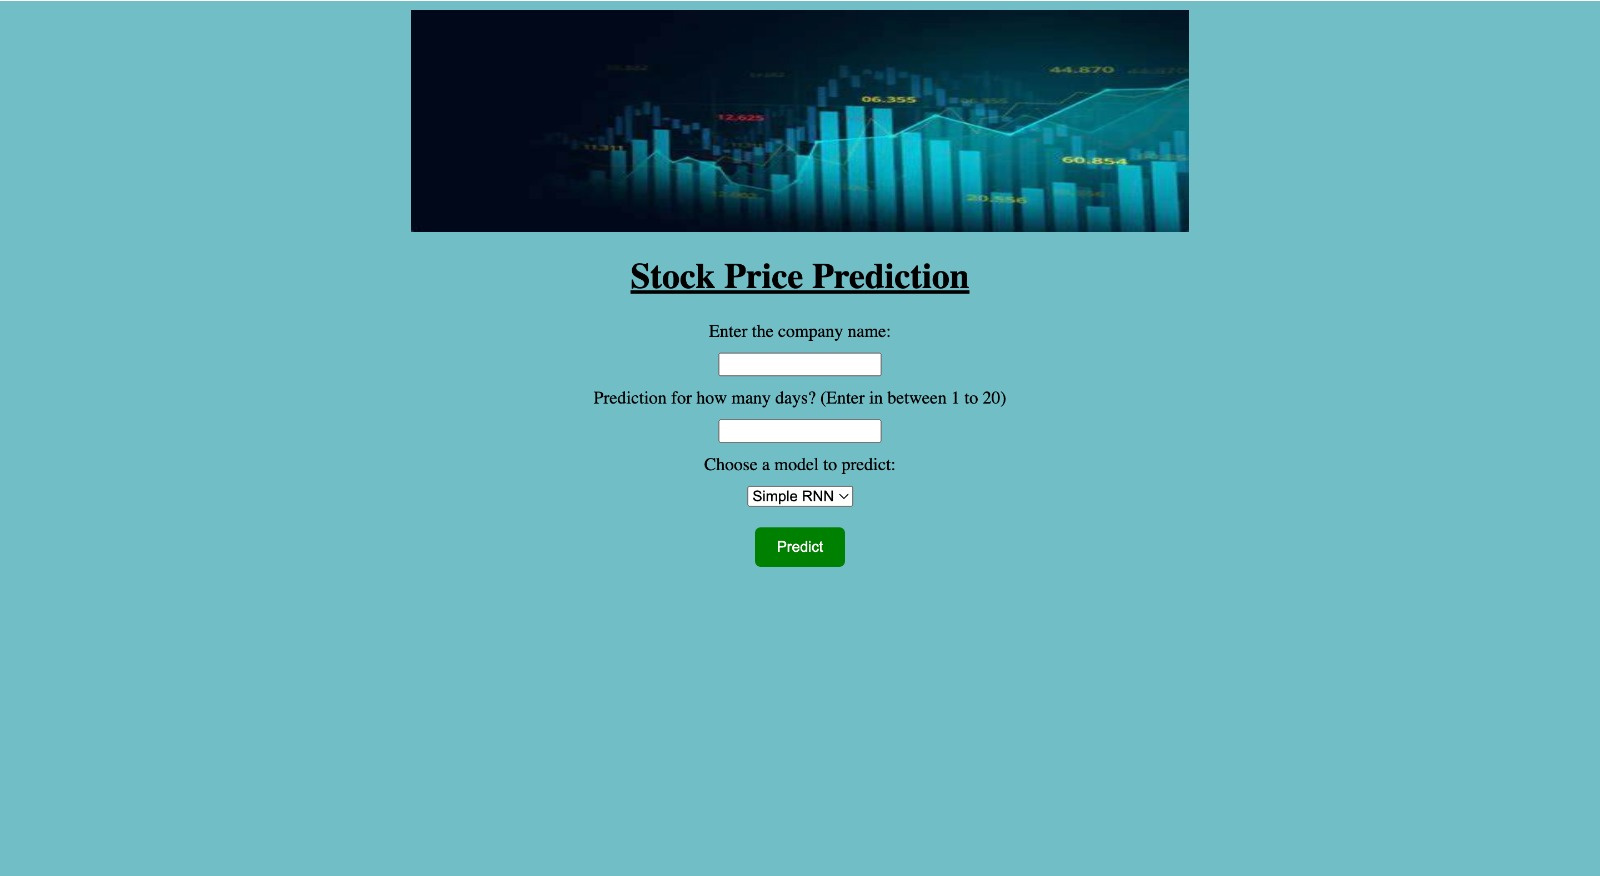
\includegraphics[width=10cm]{GOOGL_MAIN.jpg}
    \caption{Main UI page for Google}
\end{figure}
\begin{figure}[htp]
    \centering
    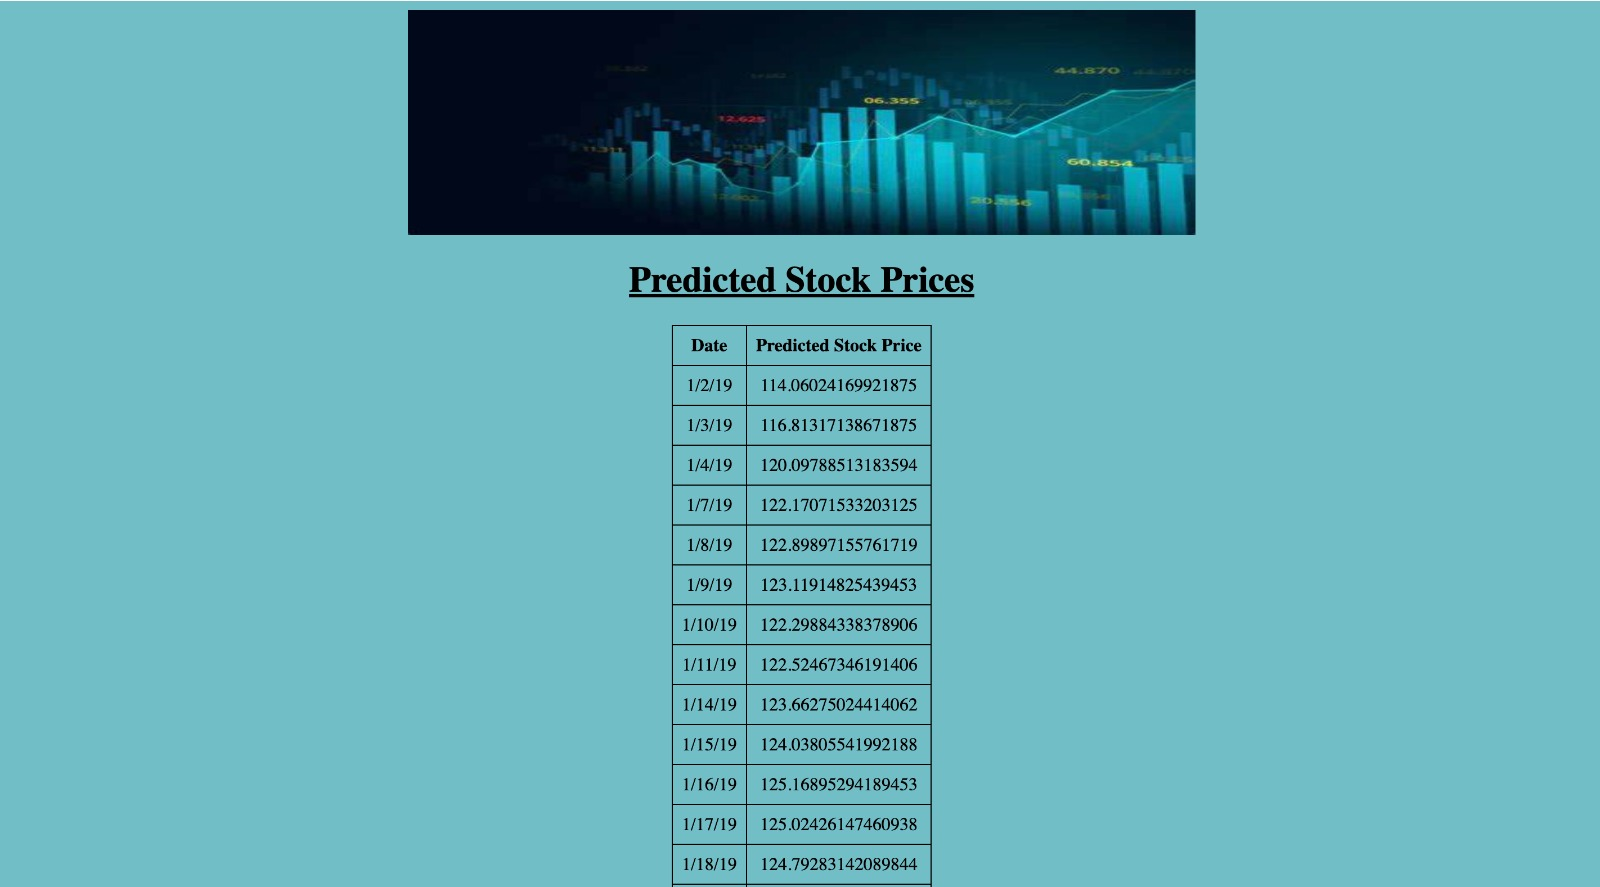
\includegraphics[width=10cm]{GOOGL_PRED.jpg}
    \caption{Predictions for Google for selected model}    
\end{figure}

\section*{References}
{
\small

[1] Sepp Hochreiter \ \& Jurgen Schmidhuber (1997). Long Short-Term Memory

[2] Andrej Karpathy \ (2015, May 21) The unreasonable effectiveness of recurrent neural networks. 

[3] Christopher Olah (2015, August 27). Understanding LSTM Networks

[4] Andrej Karpathy\ \& Justin Johnson\ \& Li Fei-Fei (2015, November 17) Visualizing and understanding recurrent networks

[5] Shi Yan (2016, March 13). Understanding LSTM and its diagrams.

[6] Klaus Greff , Rupesh K. Srivastava\ \& Jan Koutn´ık\ \& Bas R. Steunebrink \ \& Jurgen Schmidhuber (2017, October 4) LSTM: A search space odyssey

}


%%%%%%%%%%%%%%%%%%%%%%%%%%%%%%%%%%%%%%%%%%%%%%%%%%%%%%%%%%%%

\end{document}